\svnkwsave{$RepoFile: siminos/baroclinic/PCnotes.tex $}
\svnidlong {$HeadURL$}
{$LastChangedDate$}
{$LastChangedRevision$} {$LastChangedBy$}
\svnid{$Id$}

\chapter{Predrag's notes}
\label{chap:PCnotes}

\section{Introduction}
\label{s:PCintro}

    \PC{the text here is taken from
        \HREF{http://en.wikipedia.org/wiki/Baroclinic}
             {en.wikipedia.org/wiki/Baroclinic},
        needs to be rewritten}
The baroclinity (baroclinicity) of a stratified fluid is a measure of how
misaligned the gradient of pressure is from the gradient of density in a
fluid, proportional to the baroclinic vector
\beq
\frac{1}{\rho^2} \nabla \rho \times \nabla p
\,,
\ee{baroclVec}
which in turn is is proportional to sine of the angle between surfaces of
constant pressure (isobaric surfaces) and surfaces of constant density
(isopycnic surfaces). Thus, in a \emph{barotropic} fluid (which is
defined by zero baroclinity), these surfaces are parallel.

When the baroclinic vector is nonzero, the sense of the baroclinic vector
is to create vorticity to make the interface level out. In the process,
the interface overshoots, and the result is an oscillation which is an
internal gravity wave. The energy source for baroclinic instability is
the potential energy in the environmental flow. As the instability grows,
the center of mass of the fluid is lowered. Baroclinic flows can be
contrasted with barotropic flows in which density and pressure surfaces
coincide and there is no baroclinic generation of vorticity. 'Baroclinic'
means that the instability is driven by density difference; 'barotropic'
means not.

Beginning with the equation of motion for a fluid and taking the curl,
one arrives at the equation of motion for the curl of the fluid velocity,
\ie\ the vorticity. In a fluid that is not all of the same density, a
source term appears in the vorticity equation whenever surfaces of
constant density and surfaces of constant pressure are not aligned. The
material derivative of the local vorticity is given by
\begin{align}
\frac{D\vec\omega}{Dt} \equiv \frac{\partial \vec \omega}{\partial t}
 + (\vec{u} \cdot \vec \nabla) \vec \omega
    =
(\vec \omega \cdot \vec \nabla) \vec{u} - \vec \omega (\vec \nabla \cdot \vec{u})
 + \underbrace{\frac{1}{\rho^2}\vec \nabla \rho \times \vec \nabla p
   }_{\mathrm{baroclinic \, contribution}}
\,,
\label{NSvorticEq}
\end{align}
where $\vec{u}$ is the velocity and $\vec \omega$ is the vorticity, $ p $
is pressure, and $ \rho $ is density). The baroclinic vector
\refeq{baroclVec} is of interest both in compressible fluids and in
incompressible (but inhomogenous) fluids. Internal gravity waves as well
as unstable Rayleigh-Taylor modes can be analyzed from the perspective of
the baroclinic vector. It is also of interest in the creation of
vorticity by the passage of shocks through inhomogenous media, such as in
the Richtmeyer-Meshkov instability.

\emph{Baroclinic instability} arises in rapidly rotating, strongly
stratified fluids.
    \PC{the sentence taken from
    \HREF{http://www.whoi.edu/fileserver.do?id=21275&pt=10&p=17233}{Woods
    Hole}, \emph{A Search for Baroclinic Structures} by Alexander E.
    Hasha (2005), \refref{Hasha05} needs to be rewritten.}
Baroclinic instability occurs when vertical shear flows driven by
horizontal temperature gradients in a rotating domain become unstable,
and large, wavelike disturbances develop that redistribute temperature
fields in a kind of horizontally slanted convection.
Whether a fluid counts as rapidly rotating is
determined by the \emph{Rossby number}, a measure of how close the flow
is to solid body rotation. A flow in solid body rotation has vorticity
that is proportional to its angular velocity. The Rossby number is a
measure of the departure of the vorticity from that of solid body
rotation. The Rossby number must be small for the concept of baroclinic
instability to be relevant.
    \PC{maybe read \refref{Hart79,Young87,vHaFrLuPr00}?
\HREF{http://www.tos.org/oceanography/issues/issue_archive/issue_pdfs/21_4/21.4_nadiga.pdf}
    {this one} might be just simple enough for me - it's highschool level.}

The term "baroclinic" refers to the mechanism by which vorticity is
generated. Vorticity is the curl of the velocity field. The
evolution of vorticity can be broken into contributions from advection
(as vortex tubes move with the flow), stretching and twisting (as vortex
tubes are pulled or twisted by the flow) and baroclinic vorticity
generation, which occurs whenever there is a density gradient along
surfaces of constant pressure.



The simplest example of a stably stratified flow is an incompressible
flow with density decreasing with height. One measures the strength of
the stratification by asking how large the vertical shear of the
horizontal winds has to be in order to destabilize the flow and produce
the classic Kelvin-Helmholtz instability. This measure is the Richardson
number. When the Richardson number is large, the stratification is strong
enough to prevent this shear instability.

The most
geophysically relevant case is a channel whose zonal length is
substantially greater than its meridional breadth. In this instance the
form of the minimum enstrophy solution is decided by the ratio of the
energy to the squared momentum. When this parameter is below a critical
value one has a parallel flow, while if this value is exceeded, the
minimum enstrophy solution is a Rossby wave.
Periodic boundary conditions
are physically motivated for a model of atmospheric dynamics, because the
mid-latitude $\beta$-plane is typically conceived as a periodic strip wrapping
around the earth. A typical wavelength for a baroclinic disturbance in
the atmosphere is about 2000 km, which leaves space for only ten to
fifteen wave periods in a complete traversal of the globe at
mid-latitudes. Nonetheless, there are physical examples of baroclinic
instability to which the large aspect ratio approximation is applicable.
For example, baroclinic instability produces eddies in ocean currents on
the scale of 200 km. In an ocean measuring several thousand kilometers
across, there is plenty of room for large scale structures to emerge.

%%%%%%% end of {en.wikipedia.org/wiki/Baroclinic} shoplifting %%%%%%%%%%%


    \PC{the text here is taken from
    \HREF{http://www.whoi.edu/fileserver.do?id=21275&pt=10&p=17233}{Woods Hole},
     Hasha report,
        needs to be rewritten}
A number of models have been used to study this phenomenon, the most well
known of which are the Charney model and the Eady model. A basic
introduction to these models and others can be found in the textbooks by
Pedlosky [9], and Gill [4]. In this analysis, we use perhaps the simplest
model exhibiting baroclinic instability. Introduced by Phillips in 1954
[10], it consists of a two-layer quasi-geostrophic flow in a rotating
channel.
% as shown in figure 1.
Phillips analyzed the linear stability of a shear flow in which the fluid
in each layer moves with a uniform zonal velocity. The basic state
differs from that of the standard Kelvin-Helmholtz instability because
rotation forces a slanting of the free surface between the two layers in
order to balance the Coriolis force on the zonal flow. Phillips found
that instability occurs when the difference between the velocities of the
two layers exceeds a critical threshold. The model can easily be modified
to include important physical effects, such as dissipation or a planetary
vorticity gradient.

In this work, the baroclinic instability is modeled by a 2-layer
incompressible viscous fluid in a channel with no-slip side walls,
periodic in streamwise direction, top layer driven by `atmospheric
stream', \ie\ a constant total streamwise volume flow per unit time. She
simply imposes uniform streamwise velocity of unit size, ignoring the
boundary condition (could use a parabolic profile). With free slip the
layers are still unstable in the same way, just the boundary behavior is
different. Oceanographers prefer no-slip, perhaps because of coastal
stream. The bottom layer is not forced, no slip, no
\HREF{http://en.wikipedia.org/wiki/Ekman_layer}{Ekman layer}
(Ekman layer models friction at the bottom; that would make sense when
she works with 50 layers, but not two). The two layers are coupled by the
difference $\Phi_2 - \Phi_1$. Laplacian of stream function is vorticity.
Each layer is computed in terms of vorticity equations as a 2-dimensional
fluid. The lower layer has higher fluid density, and they are coupled
across their interface by difference of vorticity.

In our simulation this is about factor two; it is related to the
R\"osby deformation radius $L_R$. The spanwise $y$ width is $L_R/2\pi =
1/2$. Unless the width is larger than $L_R$, no instability. The
stream-wise aspect ration is about 8.



The present work is motivated by a series of papers
by Pedlosky ([6], [7], and a paper by Romea [11] that analyzed the
nonlinear development of baroclinic instability in the Phillips model in
a number of physically interesting situations. Pedlosky's papers, in
particular, were the first to use multiscale asymptotic methods to
compute amplitude equations for baroclinic instability. In contrast to
the present effort, Pedlosky and Romea used periodic zonal boundary
conditions and were therefore investigating the nonlinear interaction of
a discrete spectrum of unstable modes. Consequently, their calculation
led to amplitude ODEs as described above.

Our
analysis of the large aspect ratio Phillips model should provide some
insight into the kinds of structures one might expect in these
situations.

%%%%%%% end of Alexander E. Hasha shoplifting %%%%%%%%%%%

    \PC{the text here is taken from the pipes/slice article,
        needs to be rewritten}
The flow to be considered is that of $N$ layers of $2D$ incompressible
viscous fluid confined within a rectangular channel, driven by a mean
unit velocity added to the top layer in the stream-wised direction.  The
Reynolds number is defined as $\Reynolds = ?U L / \nu?$, where $U$ is the
mean velocity??? of the flow, $L$ is the channel span-wise width, and
$\nu$ is the kinematic viscosity. We scale lengths by $L/2$ and
velocities by $2U$ in the \NSe\  \refeq{NSvorticEq} for $\vec{u}$, the
deviation from the laminar flow \eqv\ $U(r)=1-r^2$. Here the
dimensionless variable $\beta$ is the fractional pressure gradient,
additional to the laminar flow, required to maintain a constant mean
velocity $U$. A Reynolds number $\Reynolds_p$, based on the applied
pressure gradient, is given by $\Reynolds_p = ??$, whereas the friction
Reynolds number is $\Reynolds_{\zeit}=??$. The \NSe\ are formulated in
cylindrical-\-polar coordinates, where $(x, y, n)$ are the stream-wise,
span-wise positions and layer, respectively. The full fluid velocity
field $U(r)\hat{{\bf z}} + \vec{u}$ is represented by
$[u,v,w,p](r,\theta,z)$, with $u$, $v$ and $w$ respectively the radial,
azimuthal and stream-wise velocity components, and $p$ the pressure. In
numerical simulations no-slip boundary conditions are imposed at the side
walls and periodic boundary conditions in the stream-wise $x$ direction.
The computational domain is
\[
\bCell={(x,y,n) \in
  [0,2\pi/\alpha]\times[0,2]\times[n]}
\,,
\] where
$L=2\pi/\alpha$ is the length of the domain.

This study is conducted at $\Reynolds = ??$, with $N=2$ and
$\alpha=1.25$, corresponding to a short $L\simeq 4\times 2$-periodic
cell in
the stream-wise direction,
\begin{align}
\bCell~ &= [1,\pi,2\pi/1.25] &\approx [90, 283, 452] \;\;\;
\text{wall units}
    \label{shortPipe}
\end{align}
At
$\Reynolds = ??$ this computational cell empirically sustains
turbulence for very long times. In average the additional pressure
fraction required to support turbulence while keeping constant mass-flux
is $\langle\beta\rangle_t=0.70$, yielding friction Reynolds number
$\Reynolds_{\zeit}=90.3$.  At this Reynolds number and geometry one domain
width $2$ corresponds to about $90?$ wall units. The domain size
\eqref{shortPipe} was chosen as a compromise between the computational
preference for small domains {\em vs.} the need for the domain to be
sufficiently long to accommodate turbulent dynamics. In addition,
restricting the largest wavelength is very useful in identifying key
coherent structures characterizing turbulent dynamics\rf{HaKiWa95}.
Although the cells studied in this paper are short, the two-dimensional
states explored here  by \eqva\ and their unstable manifolds are
strikingly similar to typical states in longer domains.

% \subsection{Numerical discretization}
% \label{s:NumDiscr}

A choice of a basis set for function space of solutions is greatly aided
by the symmetries of the flow. Baroclinic domains are stream-wise (in
numerical work) periodic, so deviation velocity field $\vec{u}$ and
deviation pressure in the \NS\ equations \refeq{NSvorticEq} are
expanded in Fourier modes in the stream-wise and span-wise directions,
\beq
\vec{u}(x,y,n) = \sum_{|k|<K} \sum_{|m|<M} \vec{u}_{nkm}
\, \mathrm{e}^{\mathrm{i}(\alpha x z+ m y)}
\,,
\ee{pipeDiscr}
whereas $N$ layers are used in the vertical direction.
Flow states are typically characterized by the instantaneous kinetic
energy of their deviation from laminar flow, $E = \frac{1}{2}
\Norm{\vec{u}}^2$, and energy dissipation rate $D =
1/\Reynolds\Norm{\bnabla \times \vec{u}}^2$. The dissipation rate is
balanced by the energy fed into the flow as
\beq
\dot{E}=I-D
\,,
\ee{Power=I-D}
where
\(
I =\oint dS \, ({\bf n}\cdot\vec{u})\, p
\)
is the additional instantaneous external power required to maintain
constant flux, over that of the laminar flow.  For \reqva\ the kinetic
energy is constant and so $D=I$, such solutions sit on the diagonal in
\reffig{f:drivedrag}, whereas for relative periodic orbits the kinetic
energy is time-periodic, with $\timeAver{D}=\timeAver{I}$ only for
long-time averages.
    \PC{
    It would be instructive to supplement $(I,E)$,
    % \reffig{fig:M1Orb},  \reffig{heterodissRPO}
    by the $(I,D)$  plot as well
    }

\section{Energy, dissipation, etc.}
% Predrag extracted this from unpublished siminos/blog/flotsam.tex
% Predrag moved this to thesis from blog/flotsam.tex jun 26 2008
%        and back again                              oct  2 2009

\subsection{Energy transfer rates, \KS}
\label{sec:energy}

This section contains material copied from \refref{SCD07},
temporarily here for inspirational purposes only.

The \KS\ [henceforth KS] system\rf{ku,siv},
which arises in the description of
stability of flame fronts, reaction-diffusion systems and many other
physical settings\rf{KNSks90}, is one of the simplest nonlinear PDEs that
exhibit spatiotemporally chaotic behavior. In the formulation
adopted here, the time evolution of the `flame front velocity'
$u=u(x,t)$ on a periodic domain $u(x,t) = u(x+L,t)$ is given by
\beq
  u_t = F(u) = -{\textstyle\frac{1}{2}}(u^2)_x-u_{xx}-u_{xxxx}
    \,,\qquad   x \in [-L/2,L/2]
    \,.
\ee{ks}
Here $t \geq 0$ is the time, and $x$ is the spatial coordinate.
The subscripts $x$ and $t$ denote partial derivatives with respect to
$x$ and $t$. In what follows
we shall state results of all calculations either in units of the
`dimensionless system size' $\tildeL$, or the system size $L = 2 \pi
\tildeL$.

In physical settings where the observation times are much
longer than the dynamical `turnover' and Lyapunov times
(statistical mechanics, quantum physics, turbulence) periodic
orbit theory\rf{DasBuch} provides highly accurate predictions
of measurable long-time averages such as the dissipation and
the turbulent drag\rf{GHCW07}. Physical predictions have to
be independent of a particular choice of ODE representation
of the PDE under consideration and, most importantly,
invariant under all symmetries of the dynamics. In this
section we discuss a set of such physical observables for the
1-$d$ KS invariant under reflections and translations. They
offer a representation of dynamics in which the symmetries
are explicitly quotiented out. We shall use these
{observables} in \refsect{sec:energyL22} in order to
visualize a set of solutions on these coordinates.

The {space average} of a function $\obser = \obser(\pSpace,t) = \obser(u(x,t))$  on
the interval $L$,
\beq
    \expct{\obser} = \Lint{\pSpace}\, \obser(\pSpace,t)
    \,,
    \label{rpo:spac_ave}
\eeq
is in general time dependent.
Its mean value is given by the {time average}
\beq
\timeAver{\obser}
    =
\lim_{t\rightarrow \infty} \frac{1}{t} \int_0^t \! d\tau \, \expct{\obser}
    =
\lim_{t\rightarrow \infty} \frac{1}{t} \int_0^t \!
    \Lint{\tau}  d\pSpace\, \obser(\pSpace,\tau)
    \,.
\label{rpo:tim_ave}
\eeq
The mean value of $\obser = \obser(u_\stagn) \equiv \obser_\stagn$ evaluated on $q$
\eqv\ or {\reqv} $u(\pSpace,t) = u_\stagn(\pSpace-ct)$ is
\beq
\timeAver{\obser}_\stagn = \expct{\obser}_\stagn = \obser_\stagn\,.
\label{rpo:u-eqv} \eeq Evaluation of the infinite time average
\refeq{rpo:tim_ave} on a function of a \po\ or \rpo\
$u_p(\pSpace,t)=u_p(\pSpace,t+\period{p})$ requires only a single
$\period{p}$ traversal,
\beq
  \timeAver{\obser}_p = \frac{1}{\period{p}}
    \int_0^{\period{p}} \! d\tau \, \expct{\obser}
\,.
\label{rpo:u-cyc}
\eeq

Equation \refeq{ks} can be written as
\beq
    u_t=- V_x
        \,,\qquad
    V(x,t)={\textstyle\frac{1}{2}}u^2+u_{x} + u_{xxx}
    \,.
\ee{ksPotent}
If $u$ is `flame-front velocity', then \expctE,
% defined in \refeq{eq:stdks},
\beq
{\textstyle\frac{1}{2}}u^2 - c u + u_x + u_{xxx}=\expctE
\,.
\label{eq:stdks}
\eeq
can be interpreted as the mean energy
density. So, even though KS is a phenomenological
small-amplitude equation, the time-dependent {$L^2$ norm
of $u$},
\beq
    \expctE=
  \Lint{\pSpace}
  V(x,t)=
  \Lint{\pSpace} \frac{u^2}{2}
  \,,
  \label{ksEnergy}
\eeq
has a physical interpretation\rf{ksgreene88} as the average `energy'
density of the flame front. This analogy to the mean kinetic energy
density for the Navier-Stokes motivates what follows.

The energy \refeq{ksEnergy} is intrinsic to the flow,
independent of the particular ODE basis set chosen to
represent the PDE. However, as the Fourier amplitudes are
eigenvectors of the translation operator, in the Fourier
space the energy is a diagonalized quadratic norm,
\beq
\expctE
          =  \sum_{k=-\infty}^{\infty} E_k
          = 2 \sum_{k=1}^{\infty} E_k
\,,\qquad
E_k =
    {\textstyle\frac{1}{2}}|a_k|^2
\,,
\ee{EFourier}
and explicitly invariant term by term
under KS translation
% \refeq{eq:shiftFour}
and reflection symmetries.
% \refeq{KSparity}.

Take time derivative of the energy density \refeq{ksEnergy},
substitute \refeq{ks} and integrate by parts. Total derivatives vanish
by the spatial periodicity on the $L$ domain:
\bea
   \dot{\expctE} &=&
     \expct{u_t \, u}
         = - \expct{\left({u^2}/{2} + {u_{x} + u_{xxx}}\right)_x u }
    \continue
    &=&
\expct{ u_x \, {u^2}/{2} + u_{x}{}^2 + u_x \, u_{xxx}}
    \,.
\label{rpo:ksErate}
\eea
The first term in \refeq{rpo:ksErate} vanishes by
integration by parts,
\(
3 \expct{ u_x \, u^2}= \expct{(u^3)_x} = 0
\,,
\)
and integrating the third term by parts yet again
one gets\rf{ksgreene88} that the energy variation
\beq
   \dot{\expctE} = P - D
                \,,\qquad
      P =  \expct{u_{x}{}^2}
                \,,\quad
      D =  \expct{u_{xx}{}^2}
\ee{EnRate}
balances the power $P$ pumped in by anti-diffusion $u_{xx}$
against the energy dissipation rate $D$
by hyper-viscosity $u_{xxxx}$
in the KS equation \refeq{ks}.

The time averaged energy density  $\timeAver{E}$
computed on a typical orbit goes to a constant, so
the expectation values \refeq{rpo:EtimAve} of drive and dissipation
exactly balance each out:
\beq
    \timeAver{\dot{E}}  =
    \lim_{t\rightarrow \infty}
        \frac{1}{t} \int_0^t d\tau \, \dot{\expctE}
=
      \timeAver{P} - \timeAver{D}
= 0
    \,.
\ee{rpo:EtimAve}
In particular, the \eqva\
and \reqva\ fall onto the diagonal in \reffig{f:drivedrag},
and so do time averages computed on \po s and \rpo s:
\beq
\timeAver{E}_p =
\frac{1}{\period{p}} \int_0^\period{p}d\tau \, E(\tau)
    \,,\qquad
\timeAver{P}_p =
\frac{1}{\period{p}} \int_0^\period{p} d\tau \, P(\tau)
    =
      \timeAver{D}_p
    \,.
\label{poE}
\eeq
In the Fourier basis \refeq{EFourier} the conservation of energy on average
takes form
\beq
0 = \sum_{k=-\infty}^{\infty} ( q_k^2 - q_k^4 )\,
    \timeAver{E}_k
\,,\qquad
E_k(t) =  {\textstyle\frac{1}{2}} |a_k(t)|^2
\,.
\ee{EFourier1}
The large $k$ convergence of this series is insensitive to the
system size $L$; $\timeAver{E_k}$ have to decrease much faster than
$q_k^{-4}$.
Deviation of $E_k$ from this bound for small $k$ determines the active modes.
For \eqva\ the $L$-independent bound
    on $E$ is given by Michaelson\rf{Mks86}.
The best current bound\rf{GiacoOtto05,bronski2005} on the long-time limit
of $E$
as a function of the system size $L$ scales as
{$E \propto L^2$}.

\subsection{Energy transfer rates for $L=22$ case}
\label{sec:energyL22}

%%%%%%%%%%%%%%%%%%%%%%%%%%%%%%%%%%%%%%%%%%%%%%%%%%%%%%%%%%%%%%%%
\begin{figure}[t]
\begin{center}
 \begin{tabular}{cc}
        ~~~~~~~~(\textit{a})                        &   ~~~~~~~~(\textit{b}) \\
    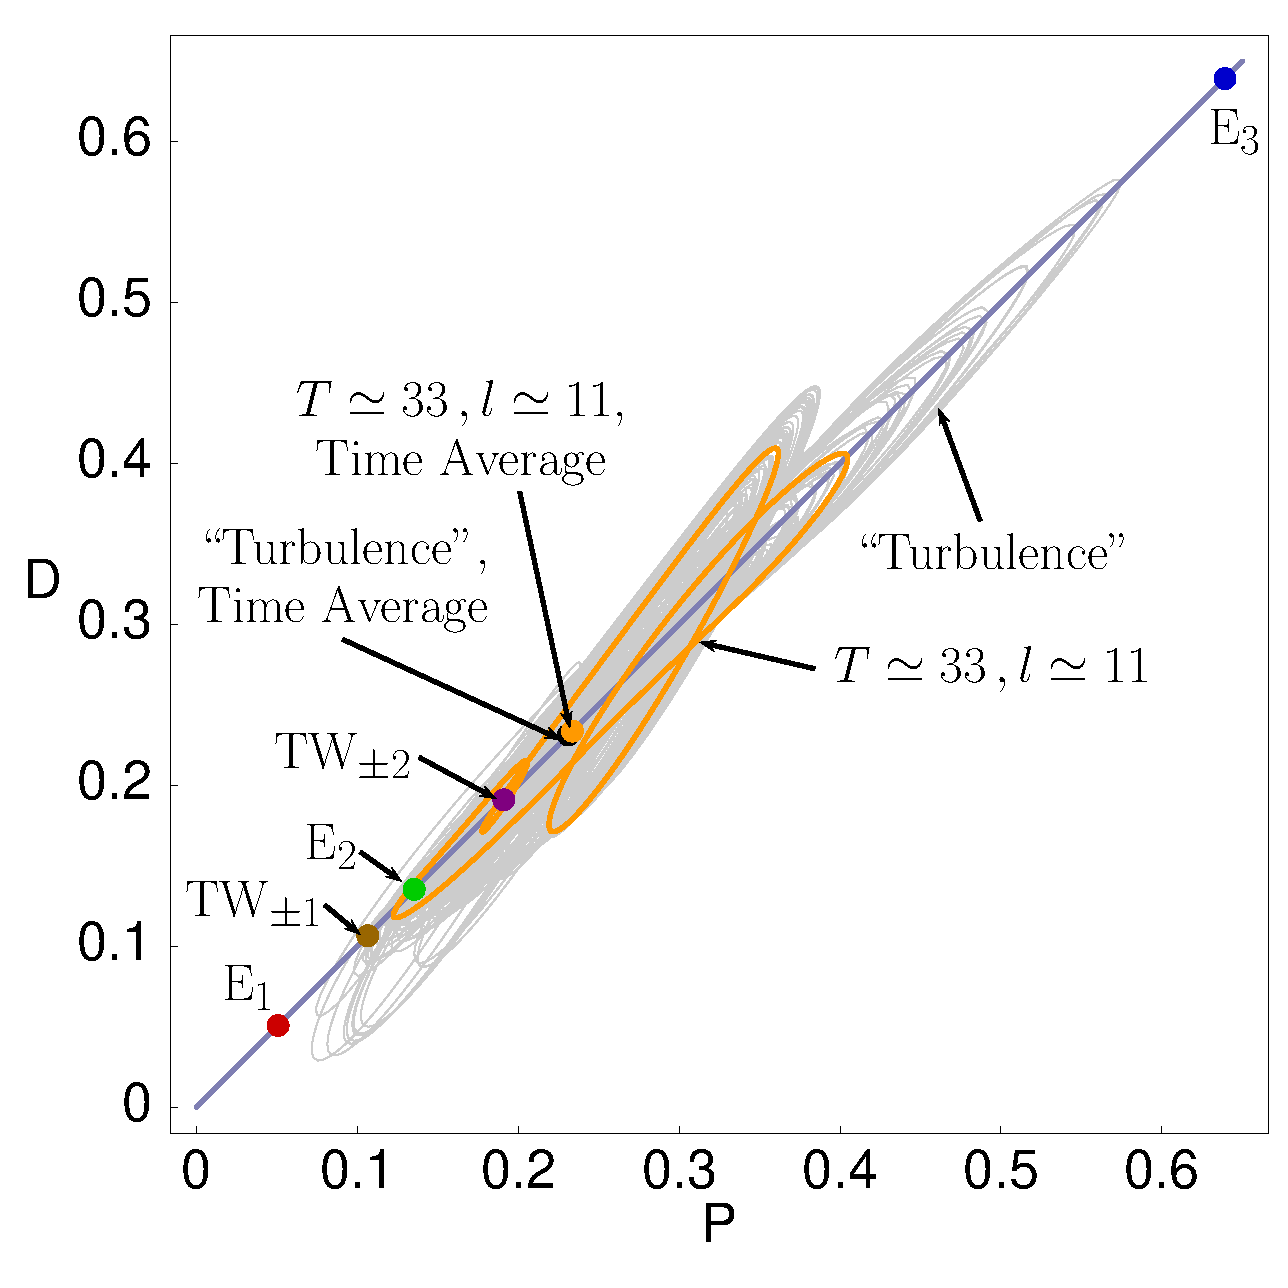
\includegraphics[width=0.46\textwidth, clip=true]{energyBalance_pst}
    & 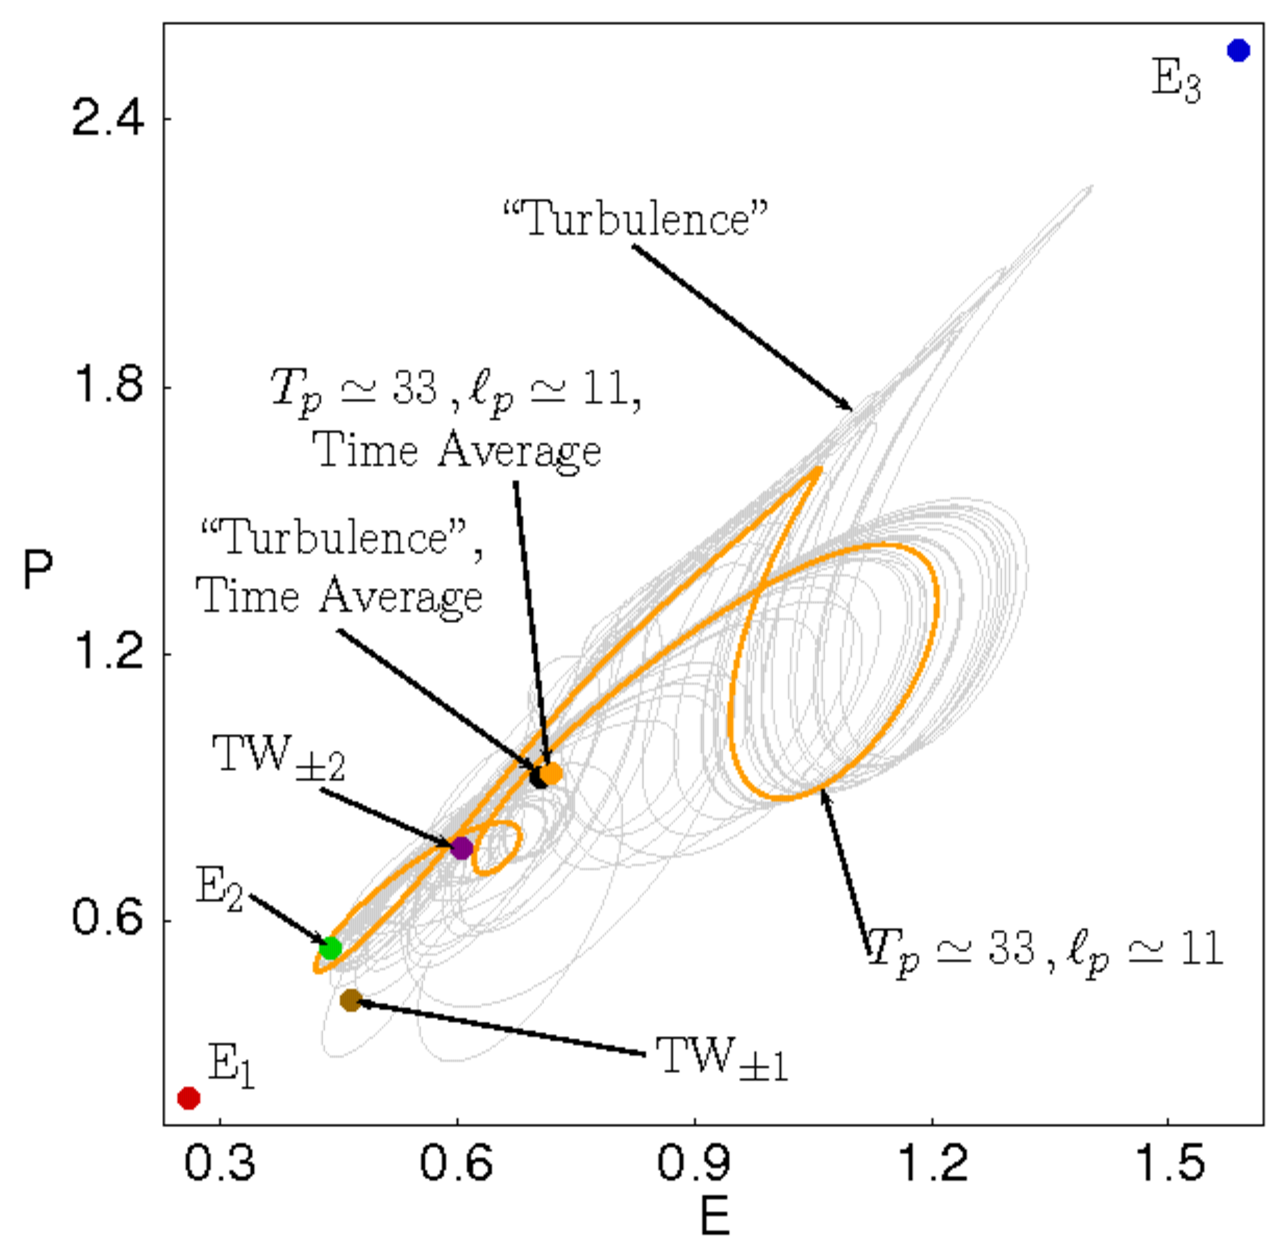
\includegraphics[width=0.46\textwidth, clip=true]{equivaEP_pst}

  \end{tabular}
\end{center}
\caption{
(a) Power input $P$ {\em vs.}
dissipation rate $D$
(b) energy $E$  {\em vs.}
power input $P$,   for several  \eqva\ and \reqva,
a \rpo, and a typical `turbulent' long-time trajectory.
System size $L=22$.
        }
\label{f:drivedrag}
\end{figure}
%%%%%%%%%%%%%%%%%%%%%%%%%%%%%%%%%%%%%%%%%%%%%%%%%%%%%%%%%%%%%%%%%%

%%%%%%%%%%%%%%%%%%%%%%%%%%%%%%%%%%%%%%%%%%%%%%%%%%%%%%%%%%%%%%%%
\begin{figure}[t]
\begin{center}
 \begin{tabular}{cc}
        ~~~~~~~~(\textit{a})                        &   ~~~~~~~~(\textit{b}) \\
    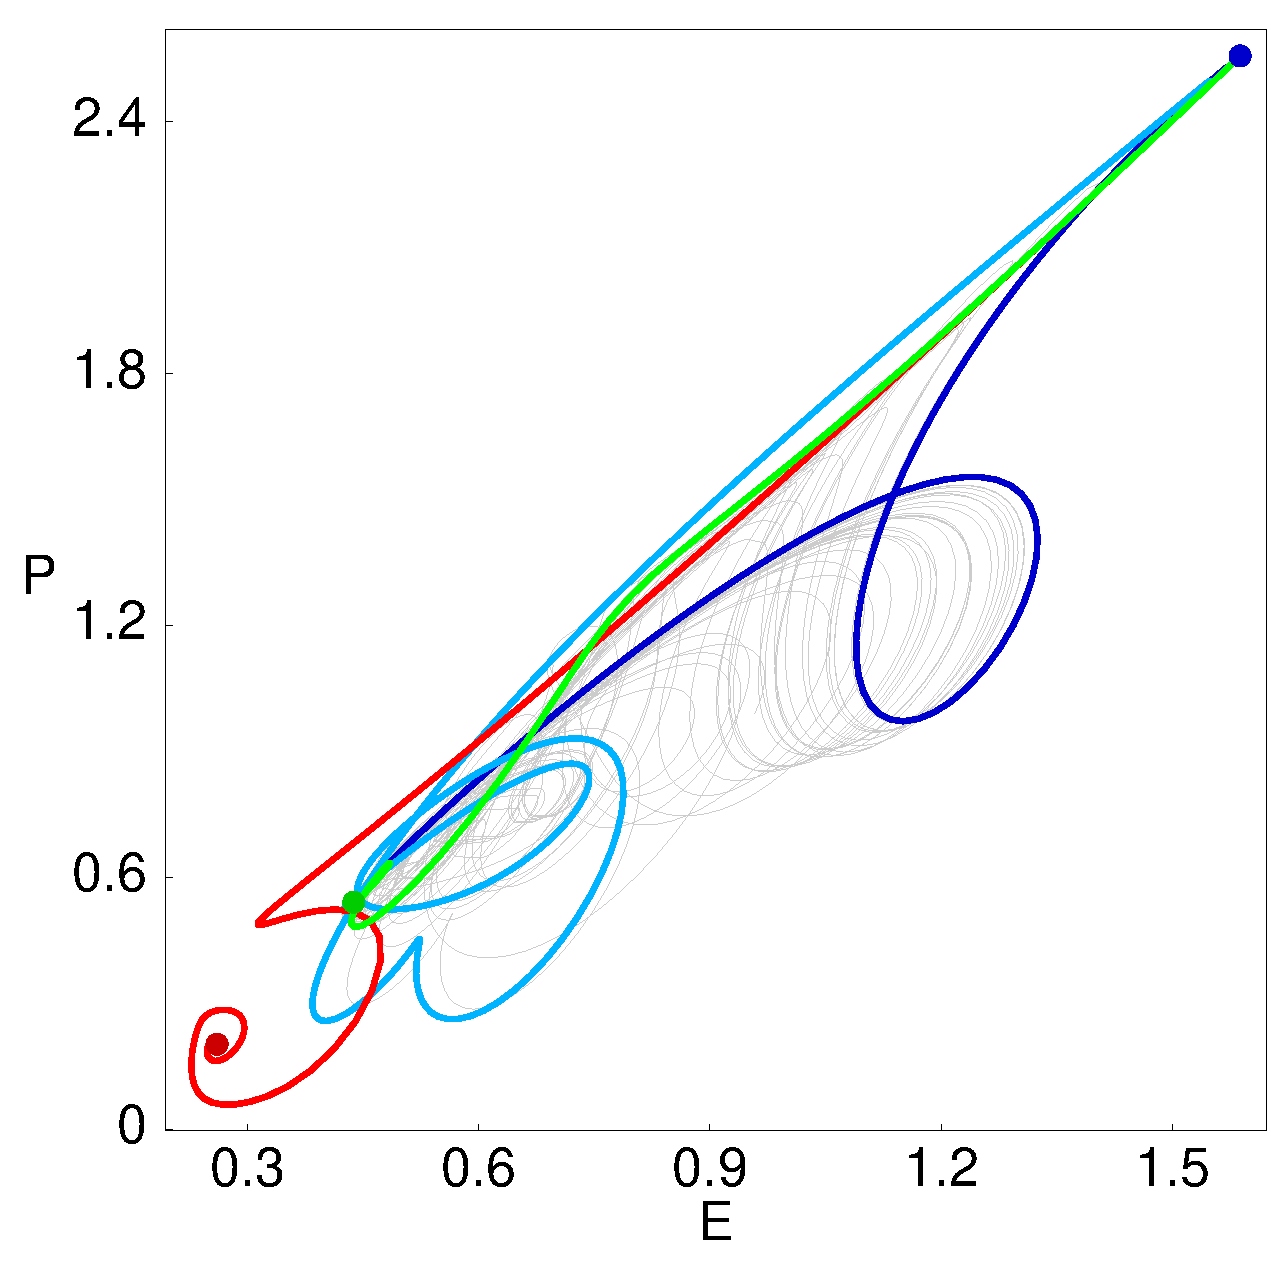
\includegraphics[width=0.46\textwidth, clip=true]{connEP}
     & 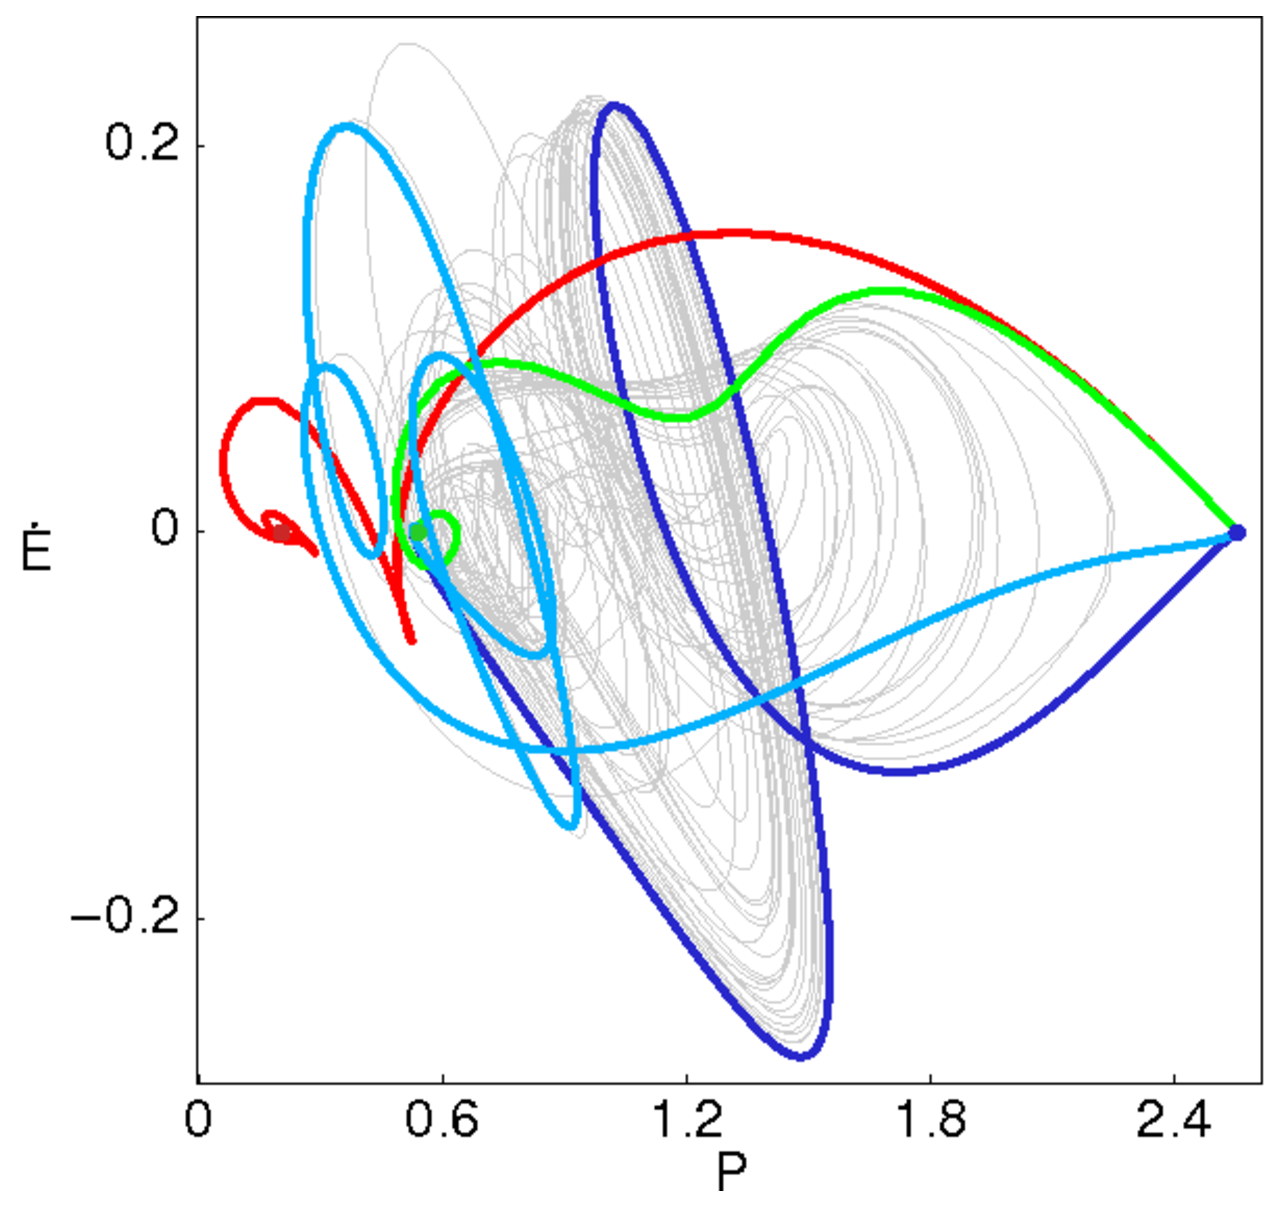
\includegraphics[width=0.46\textwidth, clip=true]{connPEdot}
 \end{tabular}
\end{center}
\caption{
Two projections of the $(E,P,\dot{E})$ representation of the flow.
\EQV{1} (red), \EQV{2} (green), \EQV{3} (blue),
heteroclinic connections from \EQV{2} to $\EQV{3}$ (green),
from $\EQV{1}$ to \EQV{3} (red)
and from \EQV{3} to $\EQV{2}$ (shades of blue), superimposed over
a generic long-time `turbulent' trajectory (grey).
System size $L=22$.
        }
\label{f:drivedragConn}
\end{figure}
%%%%%%%%%%%%%%%%%%%%%%%%%%%%%%%%%%%%%%%%%%%%%%%%%%%%%%%%%%%%%%%%%%

In \reffig{f:drivedrag} we plot \refeq{EnRate}, the time-dependent
$\dot{\expctE}$ in the power input $P$ {\em vs.}
dissipation rate $D$ plane, for $L=22$ \eqva\ and \reqva,
a selected \rpo, and for a typical `turbulent' long-time
trajectory.

Projections from the $\infty$-dimensional \statesp\ onto the 3-dimensional
$(E,P,D)$ representation of the flow, such as
\reffigs{f:drivedrag}{f:drivedragConn}, can be misleading.
The most one can say is that if points are clearly separated in an
$(E,P,D)$ plot (for example, in \reffig{f:drivedrag}
$\EQV{1}$ \eqv\ is outside the recurrent set), they are also separated
in the full \statesp.  Converse is not true -- states of
very different topology can have similar energies.

An example is the \rpo\ $(\period{p},\shift_p) = (32.8,10.96)$
% (see \reffig{f:ks22rpos}(\textit{b}))
which {is the least unstable short \rpo\ we have detected in this system.
It} appears to be well embedded within the turbulent flow. The mean power
$\timeAver{P_p}$ evaluated as in \refeq{poE}, see \reffig{f:drivedrag},
is numerically quite close to the long-time turbulent time average
$\timeAver{P}$. Similarly close prediction of mean dissipation rate in
the \pCf\ from a single-period \po\ computed by Kawahara and
Kida\rf{KawKida01} has lead to optimistic hopes that `turbulence' is
different from low-dimensional chaos, insofar that the determination of
one special \po\ could yield all long-time averages. Regrettably, not
true -- as always, here too one needs a hierarchy of \po s of increasing
length to obtain accurate predictions\rf{DasBuch}.

%%%%%%%%%%%%%%%%%%%%%%%%%%%%%%%%%%%%%%%%%%%%%%%%%%%%%%%%%%%%%%%%
\begin{figure}[t]
\begin{center}
(\textit{a})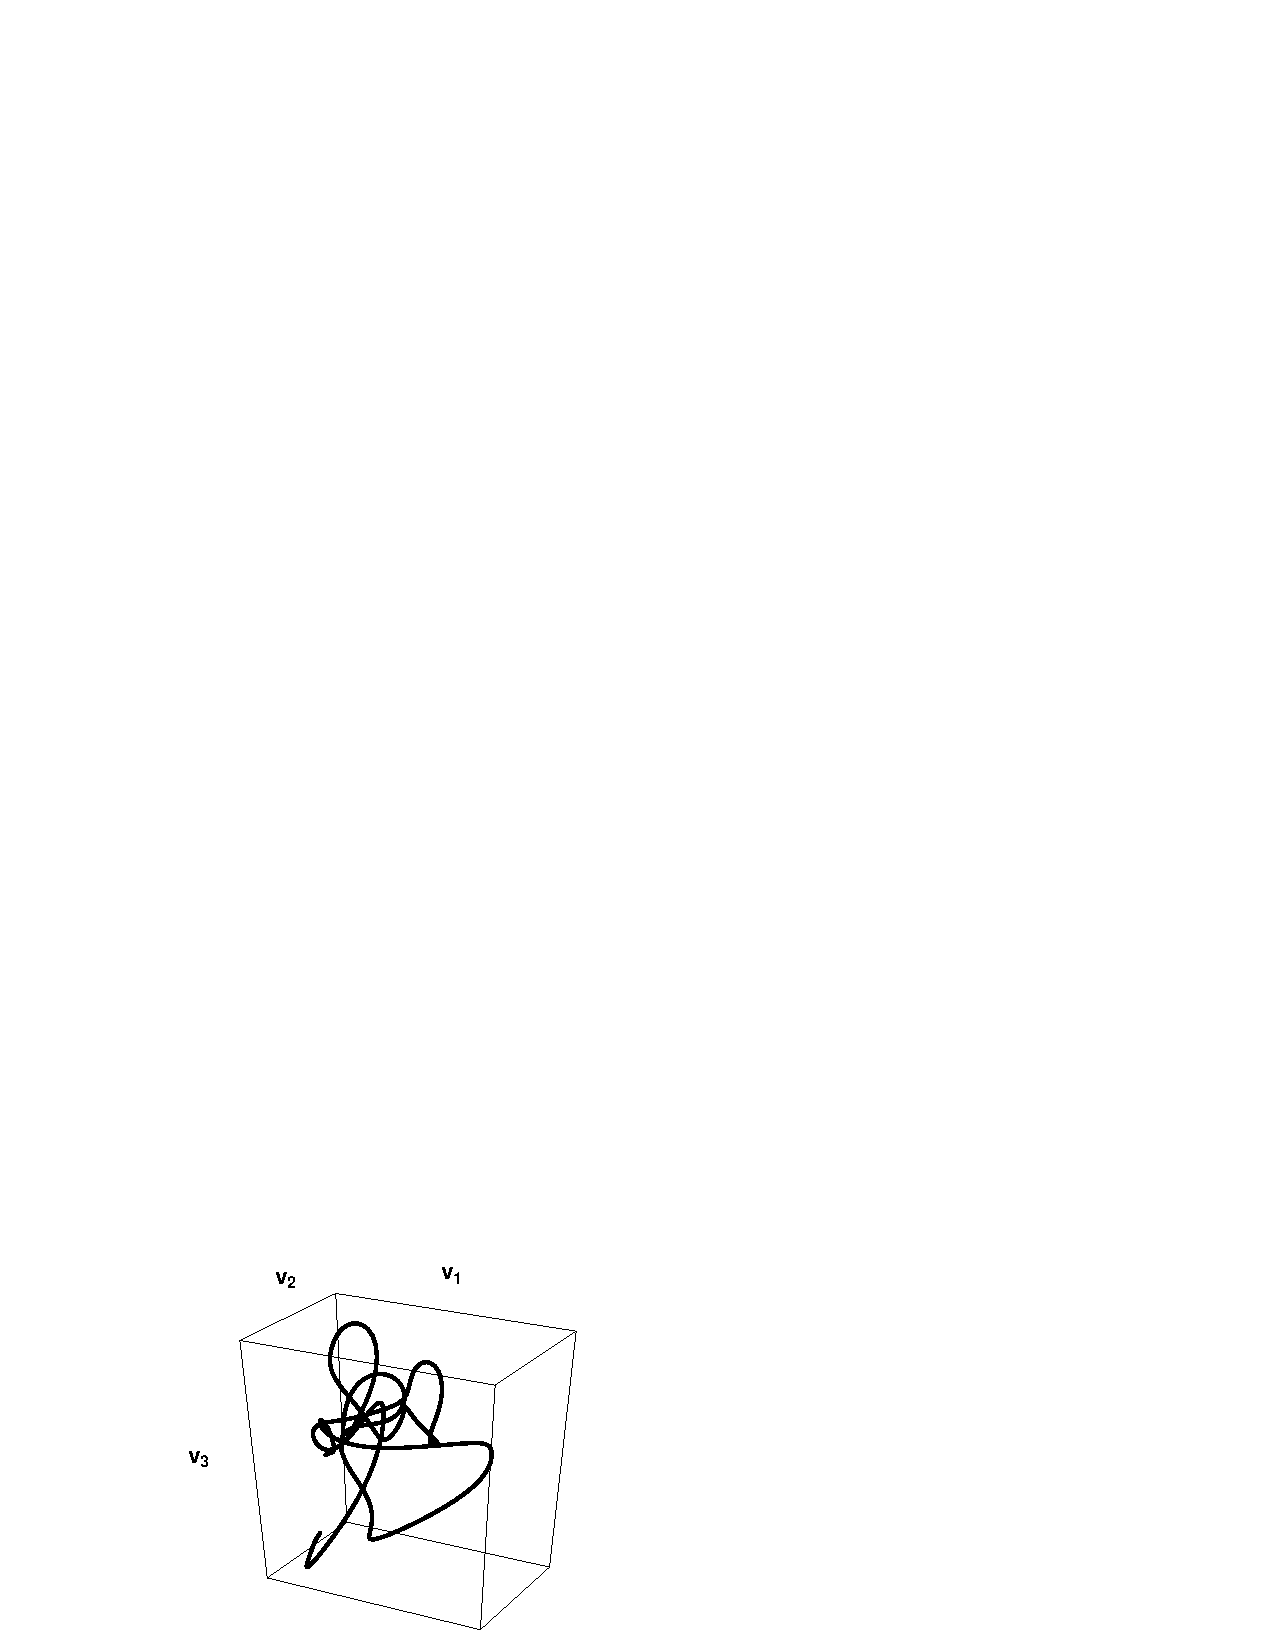
\includegraphics[width=0.46\textwidth, clip=true]{ks22rpo033p50_04p045E2}
(\textit{b})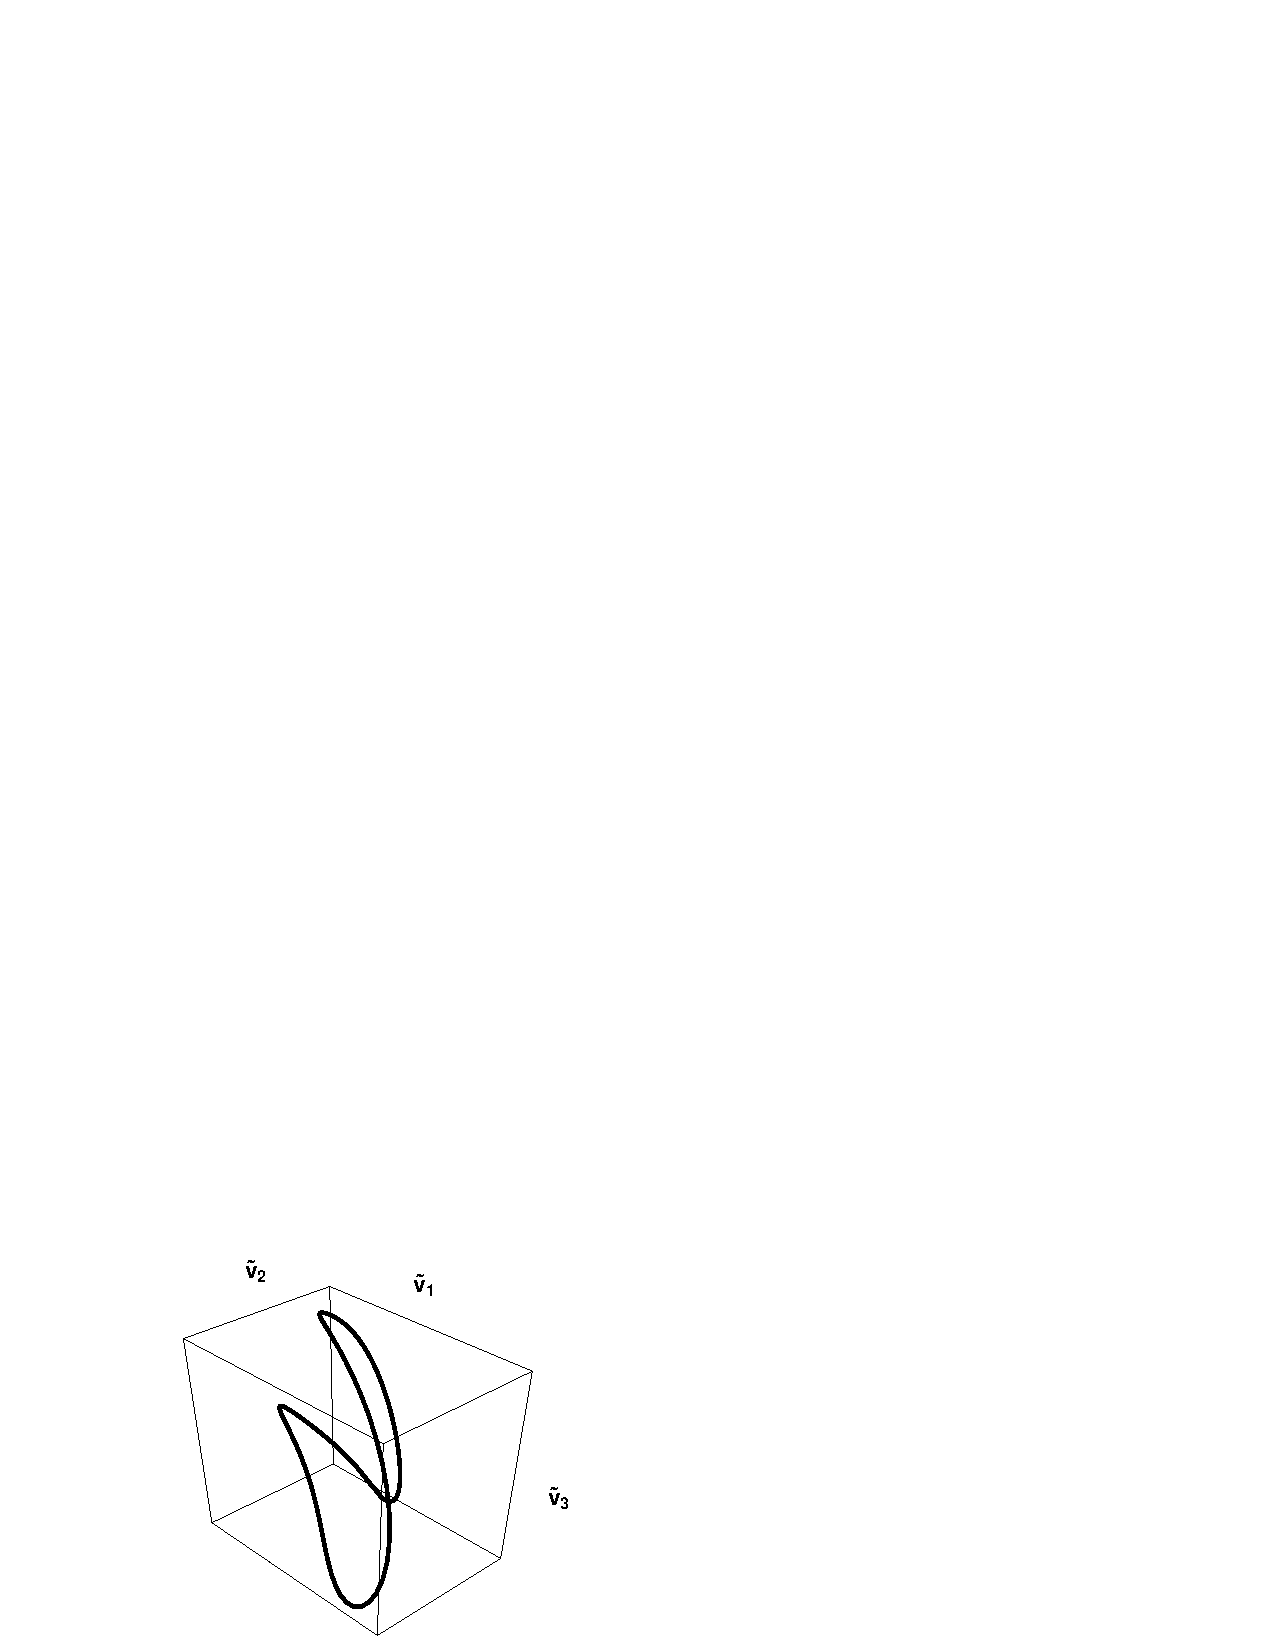
\includegraphics[width=0.46\textwidth, clip=true]{ks22rpo033p50_04p045E2CM}
\\
\end{center}
\caption{
 The
\rpo\ with $(\period{p},\shift_p) =(33.5,4.04)$
% from \reffig{f:ks22rpos}\,(\textit{c})
which appears well embedded within the turbulent flow:
 (a) A stationary \statesp\ projection,
  traced for four periods $\period{p}$.
%The coordinate axes
%$v_1$, $v_2$, and $v_3$ are those of \reffig{f:KS22E2man};
 (b) In the co-moving mean velocity frame.
%PC dropped this: traced for one period $\period{p}$.
        } \label{f:MeanVelocityFrame}
\end{figure}
%%%%%%%%%%%%%%%%%%%%%%%%%%%%%%%%%%%%%%%%%%%%%%%%%%%%%%%%%%%%%%%%%%

For any given \rpo\ a convenient visualization is
offered by the {\em mean velocity frame}, {\ie},
a reference frame that rotates with velocity
$v_p=\shift_p/\period{p}$.
In the mean velocity frame a \rpo\ becomes
a \po, as in \reffig{f:MeanVelocityFrame}\,(\textit{b}).
However, each {\rpo} has its own mean velocity frame and thus
sets of \rpo s are difficult to visualize simultaneously.

\subsection{Further observables, KS}
\label{sec:moreObs}

This section contains some material which has not been included in
publications and/or Siminos and Lan Ph.D. theses.

% from energy.tex
{\bf PC}: believe it or not, we are now set to compute
    $\timeAver{E}$ and $\timeAver{P}$
    using cycle expansions

Substitution % by \refeq{KSeqvCond}
verifies that for an \eqv\ $\expctE$ is constant:
\[
   \dot{\expctE} =
\expct{ \left({u^2}/{2} + u_{x} + u_{xxx} \right) u_x}
    = \expctE \expct{ u_x }=0
    \,.
\]


% PC worked out in part with Bridges
An infinite number of identities for moments of
solutions of KS follow\rf{Bridges_priv}. For example,
integrating by parts $\expct{u_{x} u_t}$,
$\expct{u_{xx} u_t}$,
and
$\expct{u^2 u_t}$,
respectively, one obtains \reqva\ relations
\PC{please re-derive these three. Are there more
    important ones that I have missed?
    Also, I - unnecessarily - specialized to \reqva,
    but these identities will be especially useful for \rpo s}
\RLD{I don't quite follow this process of deriving moments.  What is
the reason we look for some combinations of $u$ and its derivatives?
Why not just take $\expct{u_{x\cdots x}}$?
Is there any physical motivation for such combinations,
beyond $E$, $P$ and $D$?  Maybe use things like $\dot{P}$,
$\dot{D}$, etc.?}
\PC{they merit more thought and time than we have now, so let's
   pick them up after the first paper is submitted}
\bea
% \expct{u_{x} u_t}
%     \qquad \to \qquad
c P &=& \expct{u \, u_{x}{}^2}
\label{Bridges1}\\
c P  &=& \expct{u \, u_{xx}{}^2}
\label{Bridges3}
\,.
\eea
True for any solution:
\bea
% \expct{u_{xx} u_t}
%     \qquad \to \qquad
\dot{P} &=& 2P - \expct{u_{x}{}^3}  - 2 \expct{u_{xxx}{}^2}
\label{PC1}\\
\dot{D} &=& 2\expct{u_{xxxx}{}^2}
    + 5 \expct{u_{xx}{}^2 u_{x}}  - 2 \expct{u_{xxx}{}^2}
\label{PC2} \\
\dot{P} &=& 2P - \expct{u_{x}{}^3}  - 2 \expct{u_{xxx}{}^2}
\label{PC3}\\
\ddot{E} &=& \dot{P} - \dot{D} =
     2P - \expct{u_{x}{}^3}
    - 2\expct{u_{xxxx}{}^2} - 5 \expct{u_{xx}{}^2 u_{x}}
\label{PC4}\\
\frac{d}{dt} \expct{u_{x}{}^3} &=&
        3 \expct{u_{x}{}^3u + u_{xx}{}^3}
\label{PC5}
\,.
\eea
When moments such as \refeq{Bridges1} are added as
coordinate axes to \reffig{f:drivedragConn}, \reqva\ and
\rpo s are separated from \eqva\ and \po s. Furthermore,
as higher moments have more and more powers of $u$ and derivatives
$u_{xx\cdots x}$, their magnitudes should be strongly suppressed,
providing a symmetry-invariant basis set that can be safely truncated to
a finite-dimensional \statesp.
See  \refsect{sec:energyL22} for how this works out in practice.

Being close in such plot
does not mean that one is close in the \statesp\ - only point that are
distant from each other here have to be also distant in the full space.

For example, the energy of \reqva\ \REQV{\pm}{2} which
seems close to the
mean turbulent energy in reffig~{f:drivedrag} is separated
from it when plotted along the
$\expct{u \, u_{x}{}^2}$ moment, where according to
\refeq{Bridges1} it takes nonzero value $c P$.


\subsection{{\StateDsp} visualization of fluid flows}
\label{s:visualStatSp}
% \renewcommand{\ssp}{a}

Hopf\rf{hopf48} envisioned the function space of {Navier-Stokes} velocity fields as
an infinite-dimensional \statesp\ $\pS$ in which each instantaneous state
of $3D$ fluid velocity field $\bu(\bx)$ is represented as a unique point
$\ssp$. In our particular application we can represent $\ssp =
(\vec{u}_{nkm})$ as a vector whose elements are the primitive
discretization variables \refeq{pipeDiscr}. The $3D$ velocity field given
by $\vec{u}_{knm}(\zeit)$, obtained from integration of the \NS\
equations in time, can hence be seen as trajectory $\ssp(\zeit)$ in
$\approx 100,000$ dimensional space spanned by the free variables of our
numerical discretization, with the \NSe\ \refeq{NSvorticEq}
(or \KSe)
rewritten as
\beq
   \dot{\ssp} = \vel(\ssp) ,
   \qquad
   \ssp(\zeit) = \ssp(0)
            + \int_0^\zeit \! \mathrm{d}\zeit' \, \vel(\ssp(\zeit'))
\,,
\ee{symbolicNS}
where the current state of the fluid $ \ssp(\zeit)$ is the time-$\zeit$
forward map of the initial fluid state  $\ssp(0)$.

In order to quantify whether two fluid states are close or far from each
other, one needs a notion of distance between two points in \statesp,
measured here as
\beq
  \Norm{\ssp-\ssp'}^2  = \braket{\ssp-\ssp'}{\ssp-\ssp'} =
%\frac{1}{V}
\int_\bCell \! d \bx \;
(\vec{u}-\vec{u}') \cdot (\vec{u}-\vec{u}')
\,.
\ee{innerproduct}
As there is no compelling reason to use this {`energy norm'}, other than
that velocity fields is what is given in a numerical computation, what
norm one uses depends very much on the application. In the study of
`optimal perturbations' that move a laminar solution to a turbulent one,
both energy\rf{TeHaHe10} and dissipation\rf{LoCaCoPeGo11} norms
have been used.  In our searches for \reqva\ and \rpo s
% (see \refsect{s:rpos})
we find it advantageous to use a `compensatory' norm.
% \refeq{compensNorm}.
\beq
   \Norm{\vec{u}}_c^2 \,=\, \braket{\vec{u}}{\vec{u}}_c
   \,=\, \frac{1}{2}\,\int_V (9\,u \cdot u + 9\,v \cdot v + w \cdot w)
        \, \mathrm{d}V
\,,
\ee{compensNorm}

Visualizations of trajectory \refeq{symbolicNS} are of necessity
projections onto two or three dimensions. A physically appealing
choice\rf{KawKida01} is to monitor the flow in terms of the
symmetry-invariant and physical energy, dissipation and power input
observables $(E(\zeit),D(\zeit),I(\zeit))$.
%as in \reffig{fig:M1Orb}\,(b).
%as in \reffig{f:drivedrag}
If two fluid states are clearly separated in
such plot, they are also separated in the high-dimensional \statesp, but
converse is not true; physically distinct states might have comparable
energies, and such plots may obscure some of the most relevant features
of the flow. Furthermore, relations such as \refeq{Power=I-D} depend on
detailed type and geometry of a given problem\rf{ksgreene88,SCD07},
and further physical observables beyond $(E(\zeit),D(\zeit),I(\zeit))$
are difficult to construct.
    \PC{add here references to \refeq{Power=I-D} derivations. Does
    Frisch\rf{ frisch} do it?}

More straightforward are projections based on choices of several Fourier
components \refeq{pipeDiscr} or other primitive basis elements as
coordinate axes for projections of the flow. They are appropriate for
small perturbations off laminar state, but such coordinate axes are (i)
arbitrary and discretization-method dependent, and (ii) point in
unphysical directions, far from turbulent states which in a highly
nonlinear flows are characterized by  many strongly coupled Fourier modes
of comparable magnitude.

Recently, Gibson \etal\rf{GHCW07} have shown that the dynamics of different regions
of {\statesp} can be elucidated more profitably by a computationally
straight\-forward choice of \emph{physical} coordinates. One identifies
several prominent states of the flow $\bu_A$, $\bu_B$, $\dots$, such as
{\eqv} states and their eigenvectors, states in whose neighborhoods the
turbulent flow spends most of the time, and from them constructs, by
Gram-Schmidt or (anti)-symmetrizations, an orthonormal basis set
$\{\be_1, \be_2, \cdots, \be_n\}$. The evolving fluid state $\bu(\zeit)$
is then projected onto this basis using the inner product
\refeq{innerproduct},
\beq
\ssp(\zeit) =(\ssp_1, \ssp_2, \cdots, \ssp_n, \cdots)(\zeit)
    \,,\qquad
\ssp_n(\zeit) = \braket{\bu(\zeit)}{\be_n}
\,.
\ee{intrSspTraj}
This low-dimensional projection can be viewed in any of the $2D$ planes
$(\ssp_m, \ssp_n)$ or in $3D$ perspective views $(\ssp_{\ell},\ssp_m,
\ssp_n)$, see \reffig{f:MeanVelocityFrame}. The {\stateDsp} portraits are
{dynamically intrinsic}, since the projections are defined in terms of
intrinsic solutions of the equations of motion, and {representation
independent}, as the inner product \refeq{innerproduct} is independent of
the numerical discretization. It is worth emphasizing that the method
affords low-dimensional {\em visualization} without any low-dimensional
{\em modeling} or dimension reduction; the dynamics are computed with
fully-resolved direct numerical simulations. Although the use of
particular \reqva\ to define low-dimensional projections
% (see \refsect{s:eqbSols})
may appear arbitrary, such a choice turns out to be
very useful when the turbulent flow is chaperoned by a few invariant
solutions and their unstable manifolds, as has been shown in other low
Reynolds number settings\rf{GHCW07}. Such visualizations are a
prerequisite to uncovering the interrelations between (the infinite
number of) invariant solutions, and constructing symbolic dynamics
partitions of \statesp\ needed for a systematic exploration of turbulent
dynamics, the key challenge that we address here for the case of turbulent
pipe flows.

% \renewcommand{\ssp}{x}
